\begin{frame}
\frametitle{Authentication vs Identity}
\begin{block}{Identity} 
The identity of somebody/something is who/what he/it is.
\end{block}
\begin{block}{Authentication} Authentication is the process of
  verification that an individual or an entity is who it claims to
  be \textit{(OWASP)}. 
\end{block}
\end{frame}

%------------------------------------------------

\begin{frame}
\frametitle{Why authentication?}

Authentication is needed when you want to transmit confidential
information, you want to be sure that your correspondant isn't
impersonated by somebody else.

Authentication by itself doesn't mean confidentiality as it doesn't
prevent eavesdropping.

\end{frame}


%------------------------------------------------
\subsection{Different means of authentication}

%------------------------------------------------
\begin{frame}
\frametitle{Passwords}

\begin{itemize}
\item The most common form of authentication
\item Password should be easily changeable
\item Peoples should have different passwords for different services
\item Complexity must be sufficient
\end{itemize}
\end{frame}


%------------------------------------------------

\begin{frame}
\frametitle{Password complexity}

Enforcing a minimum password strength:
\begin{itemize}
\item State the rules clearly(e.g. minimum 10 character, minimum a
  capital letter, \ldots)
\item Check the complexity in the browser to prevent him to submit a
  form with an ``invalid'' password
\item Check again on the server side
\item If the password doesn't comply, give all the violated rules in
  the error message.
\end{itemize}

\begin{figure}
  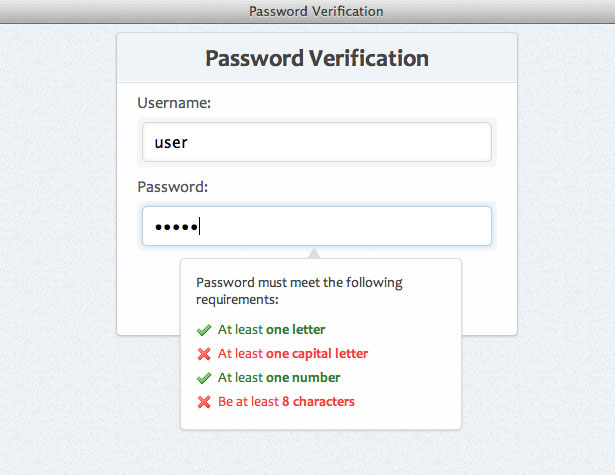
\includegraphics[width= 0.3\linewidth]{img/browserPasswordValidation.jpg}
\end{figure}

\end{frame}

%------------------------------------------------


\begin{frame}
\frametitle{One time passwords}

One time password (OTP for short) are passwords which are valid only
once. 
\begin{itemize}
\item Prevent replay attack.
\item Main difficulty: giving the user his passwords. 
\item Often cause logistical problems 
\item Used mainly by those who can afford big infrastructure (States,
  banks, other big companies, \ldots)
\end{itemize}
\end{frame}

%------------------------------------------------

\begin{frame}
\frametitle{One time passwords: choosing and distribution}

To avoid prediction, passwords must be chosen using a randow or at
least pseudorandom way.

There are various ways to distribute OTPs:
\begin{itemize}
\item If OTP generation is time based. Password are only valid for a
  short time. The generation can be done by a small electronic
  device which can be carried by the user.
\begin{figure}
  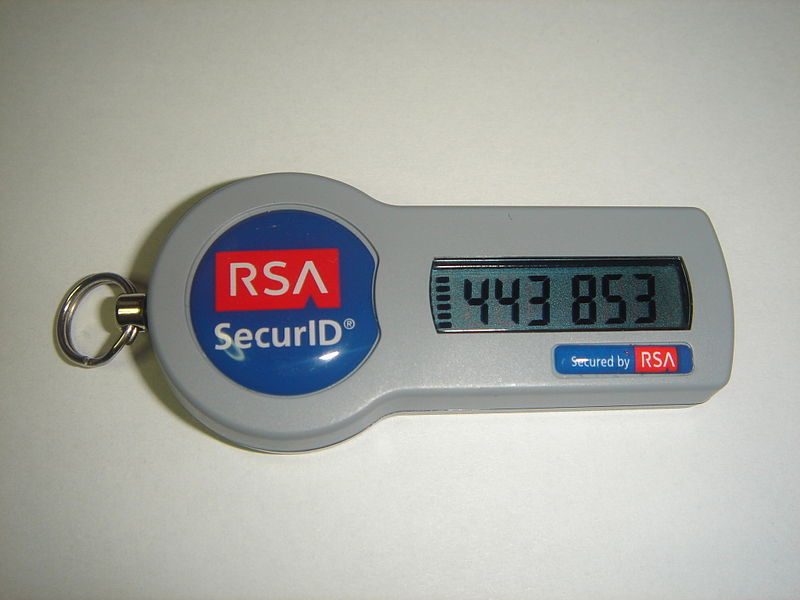
\includegraphics[width= 0.3\linewidth]{img/SecureID_token_new.JPG}
\end{figure}
\item You can send them out-of-band to the user (by SMS, mail, \ldots)
\item You can use a software on mobile phone that generate the passwords
\end{itemize}
\end{frame}

%------------------------------------------------

\begin{frame}
\frametitle{Certificates}
A trusted authority (Certification Authority) issues certificates to
confirm the ID of something. Those certificates may be of varying
quality and are most often used in SSL/TLS by web browsers.
\begin{figure}
  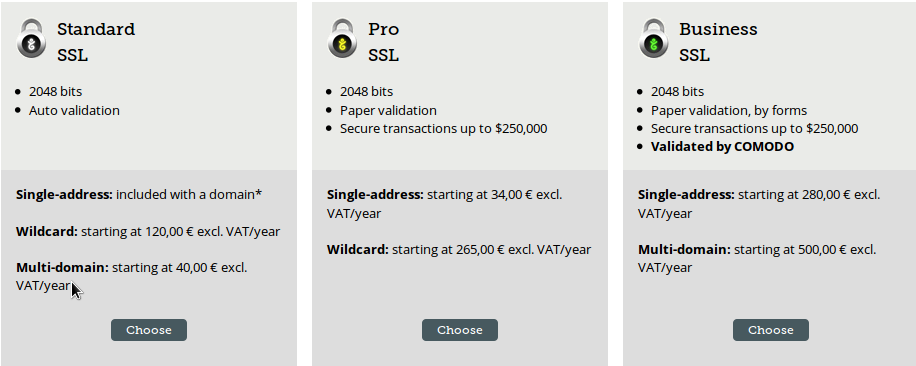
\includegraphics[width= 0.8\linewidth]{img/certificatesVariety.png}
\end{figure}
\end{frame}

%------------------------------------------------

\begin{frame}[fragile]
\frametitle{Certificates: What are they made of?}
Classical web certificates are using X.509 v3 standard.

\small
\begin{verbatim}

Certificate:
   Data:
       Version: 1 (0x0)
       Serial Number: 7829 (0x1e95)
       Signature Algorithm: md5WithRSAEncryption
       Issuer: C=ZA, ST=Western Cape,...
               OU=Certification Services Division,
               CN=Thawte Server CA/emailAddress=...
       Validity   
           Not Before: Jul  9 16:04:02 1998 GMT
           Not After : Jul  9 16:04:02 1999 GMT
\end{verbatim}

\end{frame}

%------------------------------------------------


\begin{frame}[fragile]

\small
\begin{verbatim}
       Subject: C=US, ST=Maryland,...
                OU=FreeSoft, CN=www.freesoft.org/emailAddress=...
       Subject Public Key Info:
           Public Key Algorithm: rsaEncryption
           RSA Public Key: (1024 bit)
               Modulus (1024 bit):
                   00:be ...:41:8f
               Exponent: 65537 (0x10001)
   Signature Algorithm: md5WithRSAEncryption
       93:5f...:68:9f
\end{verbatim}

\end{frame}
